\section{Trabajo relacionado}

En el artículo \cite{park2011texture} se implementan las tres etapas de un sistema de seguimiento nombradas anteriormente. Cada una de estas etapas es abordada de distintas maneras según la literatura actual.
La etapa de entrenamiento consiste en obtener una representación tridimensional del objeto al cuál se pretende seguir. En el artículo \cite{drummond1999real} se utiliza un entrenamiento off-line que consiste en obtener un modelo CAD (computer-aided design) del objeto que se desea seguir. Luego, en el artículo \cite{park2011texture} se presenta una etapa de entrenamiento novedosa que se realiza de manera on-line, en donde utiliza un marcador conocido para definir las coordenadas de los objetos y calibrar la cámara.

La etapa de detección tiene como objetivo obtener la ubicación del objeto a seguir en un frame dado. En el artículo \cite{park2011texture} utilizan el método propuesto en \cite{hinterstoisser2010dominant} para detección de objetos en imágenes 2D y lo extienden para estimar la pose 3D. Otros métodos conocidos en la literatura son los propuestos en \cite{brunelli2009template,korman13fast}. 

La etapa de seguimiento 3D cuadro a cuadro es la más importante y de la que depende el éxito o fracaso de todo el sistema de seguimiento. En el artículo \cite{park2011texture} utilizan el algoritmo ``Iterative Closest Point'' (ICP) propuesto en \cite{zhang94icp,besl92icp}, refinando el resultado con datos de bordes tomados durante la fase de entrenamiento. El método utilizado por \cite{drummond1999real} se basa en la detección de bordes para realizar el seguimiento frame a frame.

\section{Base de datos RGB-D}\label{base_rgbd}
Durante el desarrollo de este trabajo se utilizaron datos de imágenes RGB-D anotados para aplicar los métodos estudiados y tener una referencia para hacer comparaciones y sacar conclusiones sobre su eficacia. Los datos fueron tomados del trabajo \cite{lai2011large} en donde se creó una base de objetos y escenas anotada frame a frame. Esta base cuenta por un lado con varias escenas. Cada una de ellas consta de varios frames RGB con su respectiva información de profundidad. Además, la base provee información frame a frame de qué objetos aparecen y cuál es su ubicación en el plano RGB.

Por otra parte, la base provee imágenes RGB de los objetos anotados frame a frame en las escenas antes mencionadas. Para tomar estas imágenes los objetos fueron posados en una base circular giratoria y manteniendo la cámara en una posición fija se tomaron muestras con cierta regularidad cubriendo toda la circunferencia de cada objeto. Esto se hizo además desde distintas alturas permitiendo apreciar la profundidad del objeto y así obtener una mejor descripción del mismo. Cada una de estas imágenes es acompañada además por una máscara que segmenta al objeto buscado y la información de profundidad (nube de puntos) del objeto segmentado.

Los objetos elegidos para esta base se organizaron de una manera jerárquica tomada de las relaciones hiperónimo/hipónimo de WordNet. Cada objeto pertenece a una clase de objetos y hay varias instancias por cada clase. Por ejemplo, en la categoría ``taza'' existen varias instancias diferentes, que se corresponden simplemente a distintas tazas ya sea por forma o por color.

Existen distintas escenas que contienen a los objetos mencionados y en cada escena se combinan distintas clases de objetos y distintas instancias de la misma clase. De esta manera la base otorga la posibilidad de generar algoritmos capaces de identificar instancias de objetos particulares o familias de objetos según la clasificación antes mencionada.


\section{Alignment prerejective}\label{alignment_prerejective}

\section{Iterative Closest Point (ICP)}

\section{Esquema de seguimiento}
Cosas a escribir:
\begin{itemize}
	\item cómo separé las etapas en el código y por qué
	\item cómo se "comunican"
\end{itemize}


\section{Método propuesto}\label{metodo_propuesto}
Tomando como base las etapas antes mencionadas, proponemos distintos métodos para cada una de ellas. La primera etapa del sistema puede ser prescindible si contamos con el modelo 3D del objeto a seguir y una cámara calibrada. Este es el caso de estudio de esta tesis, ya que, con el propósito de poder evaluar cuantitativamente el seguimiento de objetos en secuencias de imágenes RGB-D, utilizamos la base de datos descripta en la sección \ref{base_rgbd}.
Para esta primer etapa existen varias posibilidades distintas que van desde utilizar una única nube de puntos hasta generar un modelo completo del objeto 3D alineando todas las nubes de puntos disponibles en la base. La tarea de generar un modelo completo excede el tema de estudio de esta tesis. Además el modelo resultante se utilizara únicamente para la etapa de detección por lo que se optó por el método más simple que es tomar una nube de puntos cualquiera del objeto a seguir como modelo 3D. Lo ideal sería que esta nube de puntos sea lo más completa posible, acercándose así al modelo 3D completo del objeto pero esto no es muy factible ni se puede obtener desde la base que usamos. Otra posibilidad es elegir de todas las nubes de puntos de cada objeto que otorga la base alguna cualquiera al azar. Esto resulta más realista pero sería un problema al momento de analizar los resultados ya que se agregaría una variante azarosa y se deberían correr muchas veces la misma prueba para lograr un análisis más acertado. Por estos motivos se decidió elegir una nube de puntos fija para cada objeto, en particular, la primera según orden alfanumérico del nombre del archivo proveniente de la base.


\begin{figure}
	\centering
	\begin{subfigure}[b]{0.25\textwidth}
		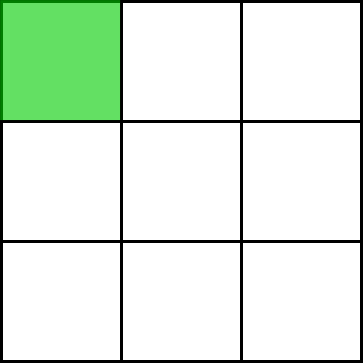
\includegraphics[width=\textwidth]{img/primercuadrante.png}
		\caption{Primer frame de búsqueda}
		\label{frames_solapados_1}
	\end{subfigure}
	\quad
	\begin{subfigure}[b]{0.25\textwidth}
		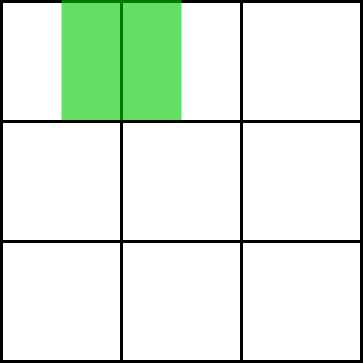
\includegraphics[width=\textwidth]{img/segundocuadrante.png}
		\caption{Segundo frame de búsqueda}
		\label{frames_solapados_2}
	\end{subfigure}	
	\quad
	\begin{subfigure}[b]{0.25\textwidth}
		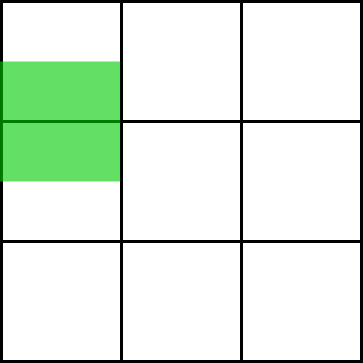
\includegraphics[width=\textwidth]{img/sextocuadrante.png}
		\caption{Sexto frame de búsqueda}
		\label{frames_solapados_3}
	\end{subfigure}
	\caption{Se busca en cada cuadrante de la grilla y en los recuadros del mismo tamaño que cubren los bordes de la grilla principal}
	\label{frames_solapados}
\end{figure}

Para la segunda etapa, la de detección, se utilizó el método descripto en la sección \ref{alignment_prerejective} refinando el resultado con ICP. La elección del mismo se realizó luego de correr varias pruebas que corroboraran la factibilidad del mismo. A través de estas pruebas se pudo observar que el método era robusto para ciertos valores de los parámetros y un objeto en particular pero que al cambiar de objeto los valores de los parámetros debían ser modificados para lograr una detección. También se observó en las pruebas que si la escena donde se buscaba el objeto era lo suficientemente pequeña, la búsqueda volvía a ser robusta no solo para un objeto en particular sino para aquellos elegidos para estas pruebas. Teniendo en cuenta esto se pensó en una variante para la detección que utilice el método elegido. Esta tenía como primer etapa obtener el alto y el ancho del modelo del objeto y multiplicarlos por un cierto valor, llamado \param{detection\_frame\_size}. Considerando estos valores dividimos la escena en cuadrantes de ese tamaño y corrimos el método de detección en cada cuadrante. Como el objeto a detectar puede haber quedado justo entre dos cuadrantes, la división se hizo de manera tal que estos cuadrantes se solapen entre si, como puede observarse en el gráfico \ref{frames_solapados} \comentarioM{Notar que la división no se hizo en el eje de la profundidad ya que las pruebas preeliminares dieron buenos resultados de esta manera y hacer eso implicaba agregarle complejidad algoritmica al método.} o \comentarioM{Notar que esta división solo se hizo en los ejes ``x'' e ``y'' y no en el eje ``z''}. La detección se corre en cada uno de estos cuadrantes y pueden suceder varias cosas:
\begin{itemize}
	\item No se encontró el objeto en ningún cuadrante: en este caso el algoritmo indica que el objeto no se encuentra en el frame
	\item Se encontró el objeto en un cuadrante
	\item Se encontró el objeto en varios cuadrantes: el algoritmo devuelve la mejor alineación encontrada
\end{itemize}

Si la detección es positiva, se refina la alineación corriendo ICP entre el modelo del objeto transformado por el método ``alignment prerejective'' y el cuadrante de la escena donde fue encontrado el mismo. Para tratar de mejorar aún más el resultado y con el objetivo de comenzar el seguimiento en las mejores condiciones posibles, se intentan tomar los puntos del objeto buscado pertenecientes a la escena. Esto se realiza porque se asume que el objeto se va modificando frame a frame, ya sea por movimientos de la cámara o del objeto. Dado que el modelo con el que se cuenta es incompleto, como se explicó en la etapa de entrenamiento, es preferible contar con el objeto de la escena en vez del modelo del objeto. Una de las formas para obtener los puntos del modelo del objeto en la escena es utilizando un k-dtree. Se arma un k-dtree con los puntos provenientes del modelo alineado y se filtran uno a uno los puntos de la escena que se encuentren cerca de al menos un punto del modelo en un cierto radio de distancia. Este valor de radio es uno de los parámetros explorados durante las pruebas, llamado \param{leaf\_size}. Los puntos que surjan de esta búsqueda son los considerados encontrados en la escena. Para que el algoritmo de búsqueda considere exitosa la detección, la cantidad de puntos filtrados de la escena debe ser mayor o igual al 50\% de los puntos del modelo original. Si todas estas etapas son superadas con éxito, se considera que el objeto fue encontrado y se pasa a la siguiente etapa, la de seguimiento. Si cualquiera de estos pasos fallara, se comienza nuevamente con la etapa de detección en el siguiente frame.

La tercera y última etapa












La detección se realizó utilizando \cite{6630856} y corrigiendo con ICP.
Cosas a escribir:
\begin{itemize}
	\item qué sucedió al tratar de detectar en toda la escena
	\item cómo se hizo para dividir la escena en partes y detectar en cada una
\end{itemize}


La utilización del algoritmo ICP \cite{zhang94icp,besl92icp} para realizar el seguimiento resulta natural e intuitiva. Por ello, es que en esta tesis se estudiará el algoritmo ICP y sus variantes \cite{estepar2004robust,segal2009generalized}, con el fin de evaluar cómo sus parámetros afectan cuantitativamente al sistema de seguimiento y la performance computacional del mismo. Asimismo, se evaluará la adaptabilidad del filtro de Kalman \cite{welch1995introduction} para seguimiento de objetos 3D en imágenes RGB-D con posibilidad de desempeño en tiempo real. El filtro de Kalman es un filtro muy popular y estudiado extensivamente en la literatura \cite{julier1997new,wan2000unscented} debido a su gran desempeño para realizar seguimiento en imágenes 2D. Por lo tanto, su aplicación en seguimiento de objetos 3D resulta de especial interés.

\section{Elección de parámetros}\label{eleccion_parametros}
\begin{table}[h]
    \begin{tabular}{|l|*{3}{c|}*{3}{c|}*{3}{c|}}
        \hline 
	    Método & \multicolumn{3}{|c|}{coffee\_mug\_5} & \multicolumn{3}{|c|}{cap\_4} & \multicolumn{3}{|c|}{bowl\_3}\\
	    \hline 
         & Over. & STD & \% foll. & Over. & STD & \% foll. & Over. & STD & \% foll. \\
        \hline
        Bhatta. ch. verde & A & A & A & B & B & B & C & C & C\\
	    \hline
	    Bhatta. x canal & A & A & A & B & B & B & C & C & C\\
	    \hline
	    Correl. ch. verde & A & A & A & B & B & B & C & C & C\\
	    \hline
	    RGB y HSV & A & A & A & B & B & B & C & C & C\\
	    \hline
    \end{tabular}
	\caption{}
\end{table}


